\chapter{Systemspiel (Taktik)}
\label{taktik}

\section{Offensive -- mit Ball}

\subsection{Abwehr (Torwart und 2er Reihe)}
\label{taktik:offensive:abwehr}

\begin{itemize}
\item Torschüsse und Pässe auf den Sturm 
\item mehrere OPtionen von einem Punkt aus
\end{itemize}

\subsubsection{Zieher}
Schräges System

\subsubsection{Pin}
\href{http://ungeblogtkickern.blogspot.de/2014/12/schusssystem-linkslang-pin-aus-der.html}{Gerades System}
(Besser wäre Rechtslang Pin)

\subsubsection{Banden}
Von Mittelpunkt



\subsection{Sturm (3er Reihe)}
\label{taktik:offensive:sturm}

Torschüsse, Duell gegen den Torwart.

\begin{itemize}
\item \href{http://ungeblogtkickern.blogspot.de/2015/11/3-punkte-theorie-auf-der-3er-reihe.html}{3 Punkte Theorie (Lücken)}
\item Mittel-Systeme
\item Lang-Systeme
\item (Drei)Viertel-Systeme
\item Systemunterschiede (Welches System das richtige für mich?)
\end{itemize}

\subsubsection{Jet Mitte}
\href{http://ungeblogtkickern.blogspot.de/2015/06/system-jet-mitte.htmli}{
Statisches Mittesystem}
\subsubsection{Pin Mitte}
\href{http://ungeblogtkickern.blogspot.de/2015/08/system-pin-mitte.html}{
Dynamisches Mittesystem}
\subsubsection{Pin Rechtslang}
\href{http://ungeblogtkickern.blogspot.de/2015/07/system-pin-rechtslang.html}{
Langes Langsystem}

\begin{figure}
%\begin{wrapfigure}{r}{0.4\textwidth} 
\centering 
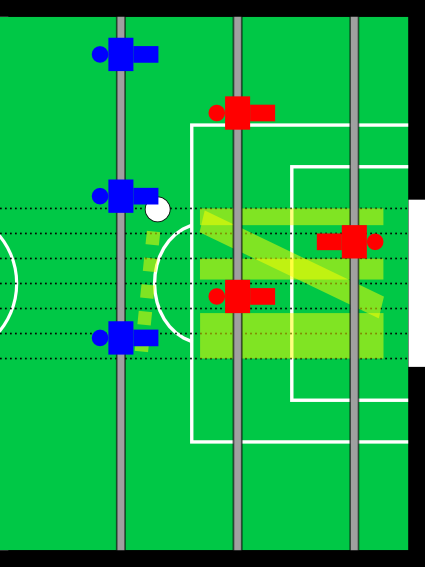
\includegraphics[width=0.25\textwidth]{img/schuss3er_lang.png} 
\caption{Rechtslang} 
\label{fig:rod-lock} 
\end{figure}
%\end{wrapfigure}

\subsubsection{Jet Linkslang}
\href{http://ungeblogtkickern.blogspot.de/2015/07/system-jet-linkslang.html}{
Kurzes Langsystem}
\subsubsection{Zieher}
\href{http://ungeblogtkickern.blogspot.de/2015/09/system-zieher.html}{
Statisches, schräges Langsystem}

 
\subsection{Passen (5er Reihe)}
\label{taktik:offensive:sturm}

\begin{itemize}
\item 2 Punkte Theorie
\item Passeigenschaften
\item http://ungeblogtkickern.blogspot.de/2015/11/passspiel-1-passeigenschaften.html
\item http://ungeblogtkickern.blogspot.de/2015/11/passspiel-2-setup.html
\end{itemize}


\section{Defensive -- ohne Ball}
\label{taktik:defensive}

Grundsätzliches
\begin{itemize}
\item Den Ball erobern für Ballbesitz und eigene Offensivaktionen. Mit den Figuren die direkten Ballwege zum Tor blockieren und den Ball annehmen/fangen. 
\item Antizipieren: Was kann passieren? Gegner lesen: Was hat der Gegner vor? (Spielart, Spielniveau, Lieblingsschuss, Entscheidung, ...)
\end{itemize}

Strategien:
,,Re-aktion'': Auf den Ball reagieren, also die Laufbahn des Balls mitverfolgen oder ,,Aktion'':
\begin{itemize}
\item Locken (Lücke)
\item Erschweren (Shuffle)
\item Kreuzen (Wegziehen)
\item Außenmann 
\item \href{http://ungeblogtkickern.blogspot.de/2015/06/defensivbewegungen-im-verteidigerbereich.html}{Artikel auf Ungeblogt}
\end{itemize}


\subsection{Abwehr: Torwart- und 2er-Reihe}
\label{taktik:defensive:halten}

3 Punkte Deckung


\subsection{Mittelfeld (5er-Block)}
\label{taktik:defensive:5erblock}

\begin{itemize}
\item Locken (Lücke)
\item Erschweren (Shuffle)
\item Zurückfahren (Wegziehen)
\item http://ungeblogtkickern.blogspot.de/2015/05/5er-defensive.html
\item http://ungeblogtkickern.blogspot.de/2015/06/defensivbewegungen-auf-der-5er-reihe.html
\item Passeigenschaften ausnutzen, Rebound
\item http://ungeblogtkickern.blogspot.de/2015/11/passspiel-1-passeigenschaften.html
\item http://ungeblogtkickern.blogspot.de/2015/11/passspiel-2-setup.html
\end{itemize}  



\subsection{Aktives Stellungsspiel}
\label{taktik:defensive:aktivesstellungsspiel}

\begin{itemize}
\item Aufbau an der 5er Reihe
\item Schräge Systeme
\item Gerade Systeme
\item Wechsel zwischen verschiedenen Systemen
\item Runterklappen Sturm und Mittelfeld
\end{itemize}
